% \chapter{Background}
\chapter{LiFi Channel and System Models}
\label{ch:ch_background}

\section{Introduction}
\label{ch:ch_background:intro}
    
    
    \lipsum[1]

    At the time of writing, \gls{tgbb} has agreed on the operating wavelength spectrum for \gls{ieee} 802.11bb.
    Based on \shortcite{tgbbcommonmode}, the related motion states the following.
        \begin{quoting}
            ``Move to adopt the 800nm - 1,000nm wavelength spectrum as the mandatory, common mode wavelength for all TGbb STAs.'' 
        \end{quoting}
    

    The first reason is that the responsivity of silicon-based \glspl{pd} is higher at those ranges compared to that in the \gls{vl} spectrum as shown in \figref{fig:ch_background:responsivity}, which shows four samples of responsivities of different Silicon-based \glspl{pd} taken from \cite{edmundoptics}.
    

        \begin{figure}
            \begin{center}
                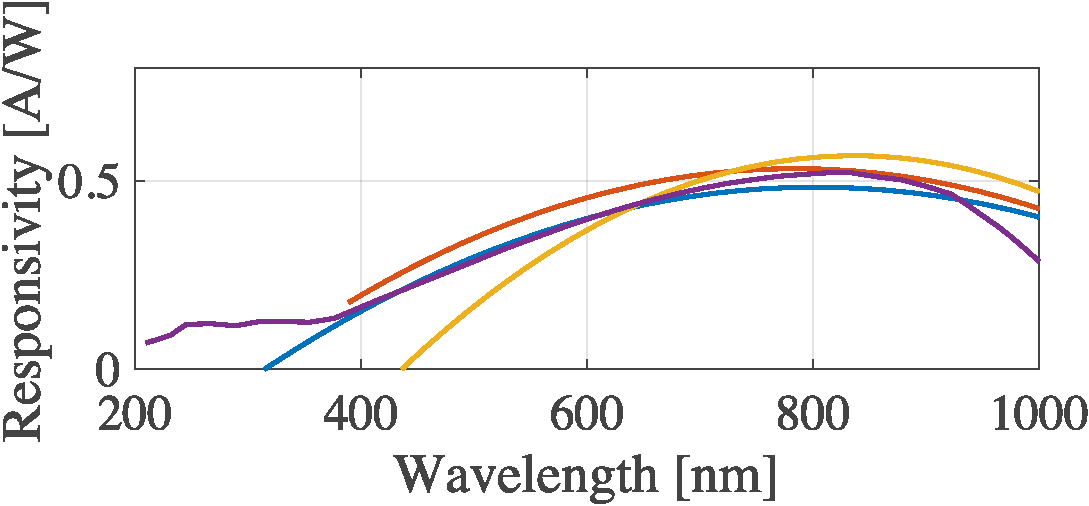
\includegraphics[width=0.5\columnwidth,draft=false]{./ch_background/figs/responsivity.pdf}
                \caption{Responsivities of four different Silicon-based \glspl{pd} taken from \protect\cite{edmundoptics}. (Please refer to \protect\cite{edmundoptics} for more detailed information on the corresponding curves. Note that details are removed for clarity purposes.)}
                \label{fig:ch_background:responsivity}
            \end{center}
        \end{figure}


    % In addition, as the downlink and uplink transmissions are assumed to occupy the \gls{vl} and \gls{ir} spectra, respectively, the comparisons of the \glspl{cir} over both spectra are worth discussing here.
    % Note that throughout this thesis, the wavelength range of 800 nm to 1,000 nm is considered when a signal is transmitter over the \gls{ir} spectrum.
    % The assumptions of the system model in this chaptesr are also used for that in the next chapters.   

    

\section{LiFi Channel Model}
\label{ch:ch_background:channelmodel}
    
% \subsection{Transmission Model}
% \label{ch:ch_background:transmissionmodel}
    
    
    Based on \cite{kahnkrause,infraredkahn}, the received optical power can be expressed as:
        \begin{align}
            y(t) = h(t) \circledast x(t),
        \end{align}
    where $\circledast$ denotes the convolution operation. 
    


\subsection{Channel Model}
\label{ch:ch_background:owcsimpy}

    
    For the sake of the illustrations, different opacities of faces in \figref{fig:ch_background:owcsimpy}(b) show different reflectivities, i.e., the head portions of the models have different reflectivities compared to the body portions of the model.
    

        \begin{figure}[h]
        \centering
        \begin{subfigure}[b]{0.49\columnwidth}
            \centering
            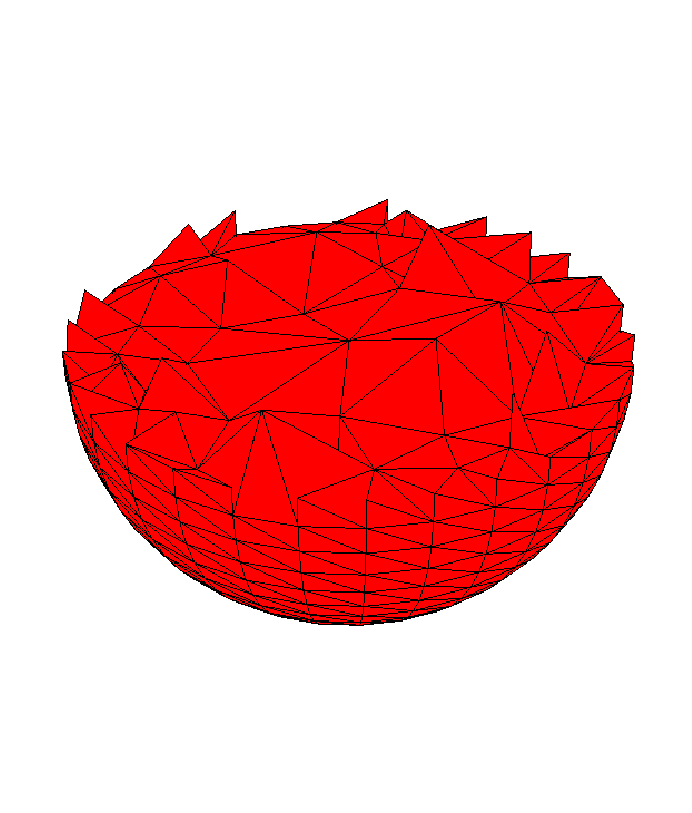
\includegraphics[width=0.5\columnwidth,draft=false]{./Appendix/figs/arb3d.pdf}
            \caption{}
        \end{subfigure}~
        \begin{subfigure}[b]{0.49\columnwidth}
            \centering
            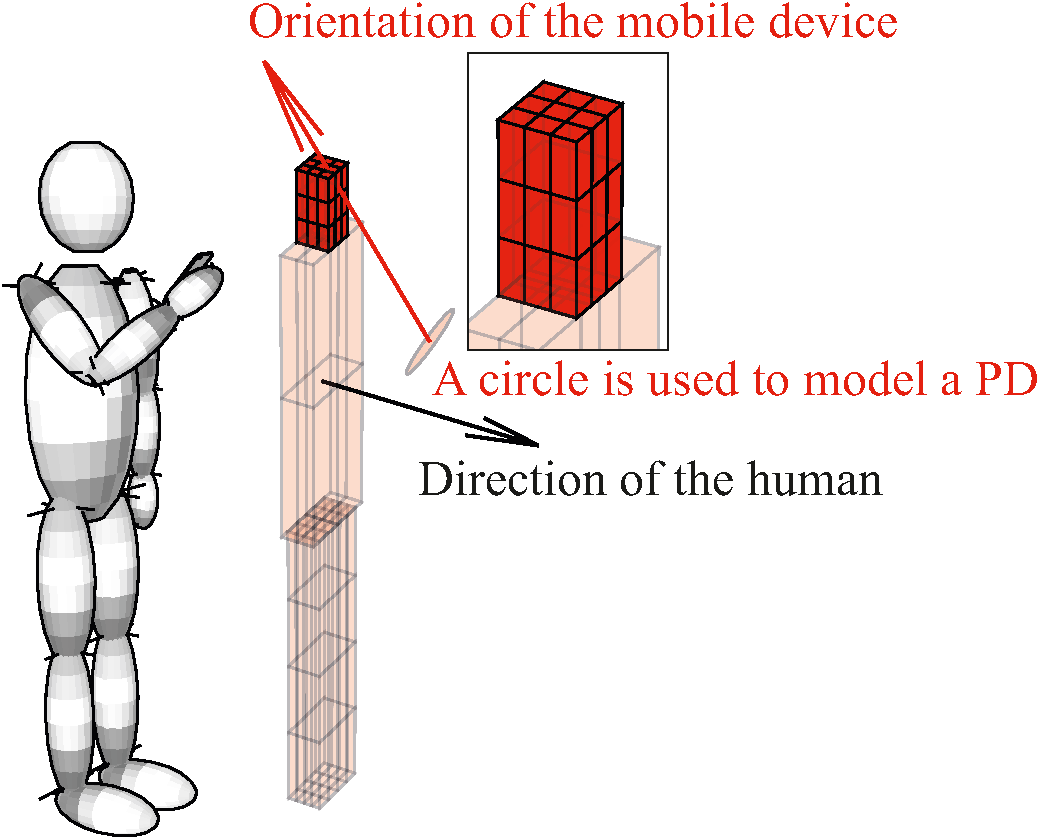
\includegraphics[width=0.85\columnwidth,draft=false]{./ch_background/figs/humanmodel_rev2.pdf}
            \caption{}
        \end{subfigure}
        \caption{(a) An example of a 3D object as a collection of 2D faces, and (b) a human model as a collection of square faces.}
        \label{fig:ch_background:owcsimpy}
      \end{figure}

    

\subsection{A Simple Office Environment}
\label{ch:ch_background:simpleoffice}

    
    
    

      \begin{table}[t]
        \caption{Reflectivities of materials over visible light (VL) and infrared (IR) spectrum.}
        \label{tab:reflectivity}
        \centering
        \begin{tabularx}{\columnwidth}{|l||Y|Y|Y|Y|c|}
        % \begin{tabular}{|l||c|c|c|c|c|}
        \hline
        Materials:               & paint & cotton & skin & plaster & pinewood \\ \hline
        Reflectivities (@ 940 nm): & 0.04               & 0.65   & 0.70 & 0.85    & 0.92 \\ \hline
        Reflectivities (@ 850 nm): & 0.04               & 0.64   & 0.66 & 0.83    & 0.92 \\ \hline  
        % \end{tabular}
        \end{tabularx}
      \end{table}

    Summaries of the reflectivities of the materials can be found in Table~\ref{tab:reflectivity}. 

    

         \begin{figure}[h]
            \centering
            \begin{subfigure}[b]{0.49\columnwidth}
                \centering
                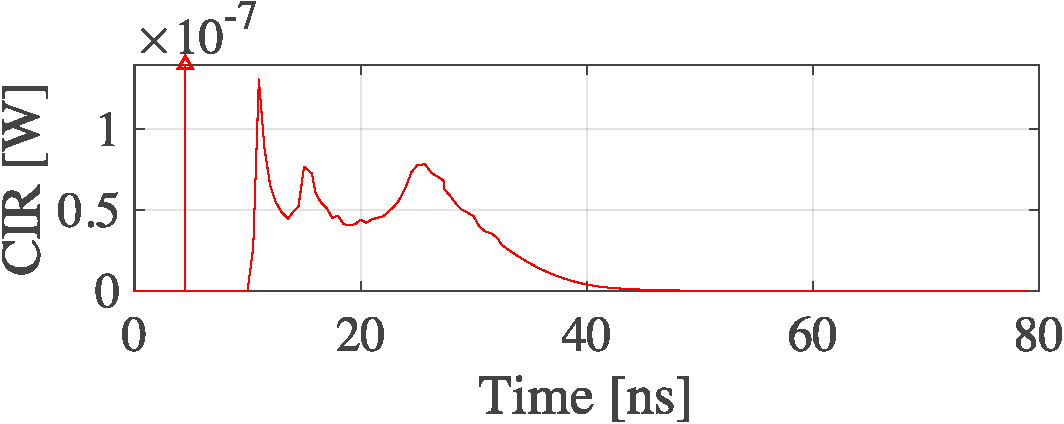
\includegraphics[width=1\columnwidth,draft=false]{./ch_background/figs/case1_ul_n.pdf}
                \caption{Case 1: 940 nm}
            \end{subfigure}~
            \begin{subfigure}[b]{0.49\columnwidth}
                \centering
                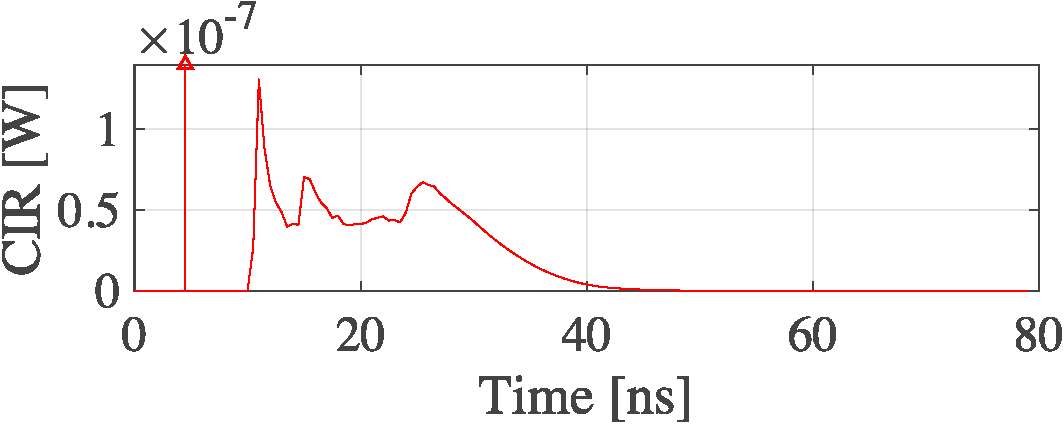
\includegraphics[width=1\columnwidth,draft=false]{./ch_background/figs/case1_ul.pdf}
                \caption{Case 1: 850 nm}
            \end{subfigure}\\
            \begin{subfigure}[b]{0.49\columnwidth}
                \centering
                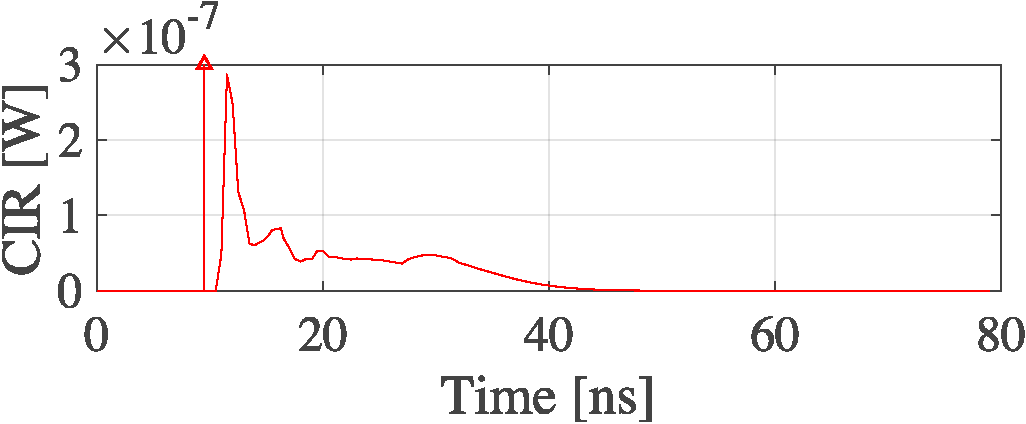
\includegraphics[width=1\columnwidth,draft=false]{./ch_background/figs/case2_ul_n.pdf}
                \caption{Case 2: 940 nm}
            \end{subfigure}~
            \begin{subfigure}[b]{0.49\columnwidth}
                \centering
                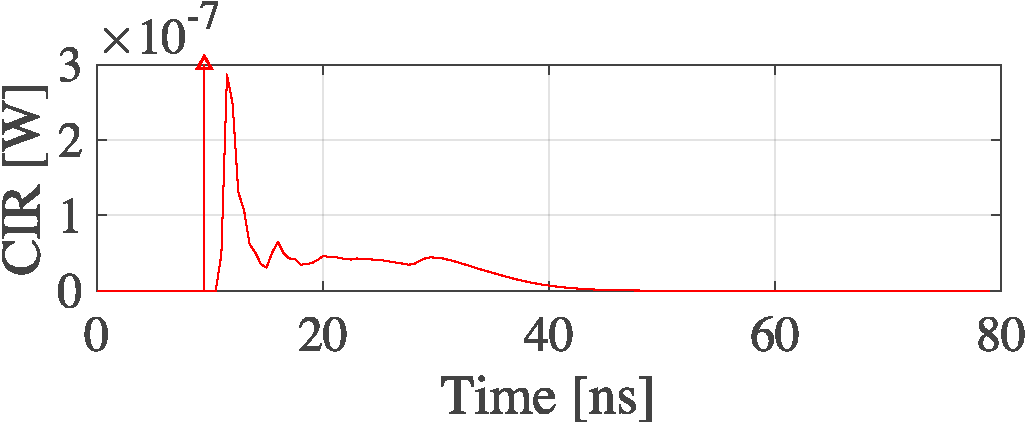
\includegraphics[width=1\columnwidth,draft=false]{./ch_background/figs/case2_ul.pdf}
                \caption{Case 2: 850 nm}
            \end{subfigure}\\
            \begin{subfigure}[b]{0.49\columnwidth}
                \centering
                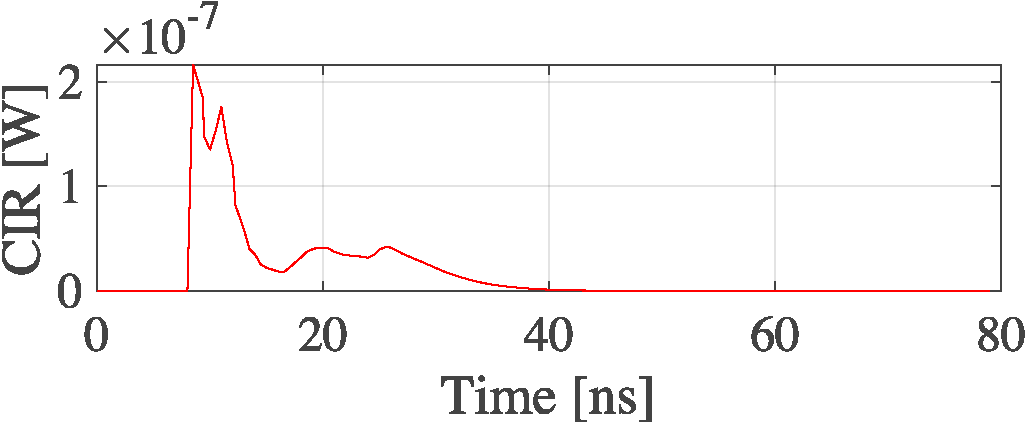
\includegraphics[width=1\columnwidth,draft=false]{./ch_background/figs/case3_ul_n.pdf}
                \caption{Case 3: 940 nm}
            \end{subfigure}~
            \begin{subfigure}[b]{0.49\columnwidth}
                \centering
                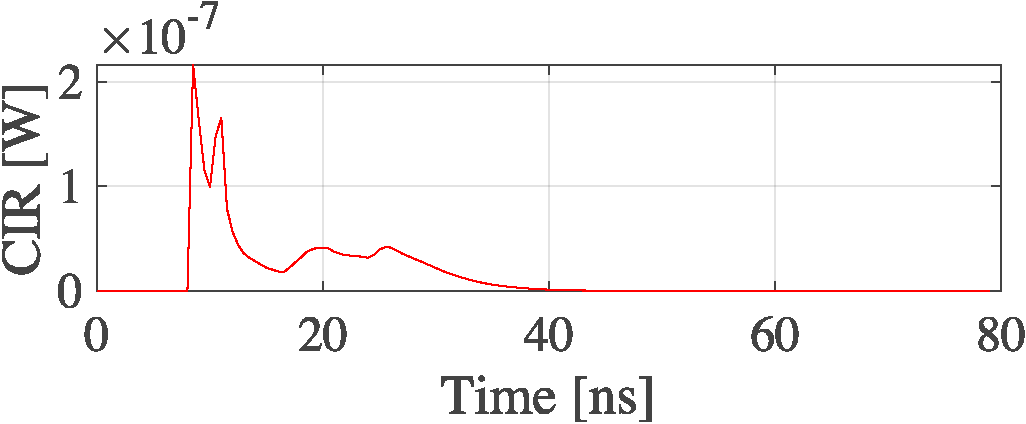
\includegraphics[width=1\columnwidth,draft=false]{./ch_background/figs/case3_ul.pdf}
                \caption{Case 3: 850 nm}
            \end{subfigure}
            \caption{CIRs.}
            \label{fig:ch_background:casesres}
        \end{figure} 

